\documentclass[11pt, a4paper]{article}

\usepackage[utf8]{inputenc}
\usepackage{graphicx}
\usepackage{hyperref}
\usepackage{geometry}
\usepackage{booktabs}
\usepackage{amsmath}
\usepackage{amssymb}
\usepackage{xcolor}
\usepackage{float}
\usepackage{setspace}
\usepackage{caption}
\usepackage{subcaption}
\usepackage{natbib}

\geometry{margin=1in}
\setstretch{1.15}

\title{\Huge \textbf{Network-Based Structural and Influence Analysis of Financial Systems} \\
\vspace{0.3cm}
\Large S\&P 500 Correlation Network}
\author{Network Science Project}
\date{\today}

\begin{document}

\maketitle

\begin{abstract}
\noindent This report presents a network-science analysis of the S\&P 500 equity market. A correlation-based financial network is constructed from two years of daily log-returns, with market-mode filtering applied to remove the dominant common factor. The resulting network is analysed for scale-free degree distributions, small-world properties, community structure, robustness, and contagion dynamics. Small-worldness is validated against both Erd\H{o}s--R\'enyi and degree-preserving configuration model baselines, with bootstrap confidence intervals ($B=200$). Three historical market events are used to empirically validate the propagation model. Rolling-window analysis tracks the temporal evolution of network topology across 18 overlapping windows.
\end{abstract}

\newpage
\tableofcontents
\newpage

% ===================================================================
\section{Introduction}
% ===================================================================

Financial markets exhibit complex interdependencies that extend beyond pairwise asset correlations. During crises, these dependencies amplify---a phenomenon variously termed contagion, systemic risk, or cascade failure~\citep{barabasi2016network}. Understanding the topology of these relationships is central to risk management, portfolio construction, and regulatory oversight.

This project constructs an undirected, weighted network of $N=501$ S\&P 500 constituents from daily price data spanning 2024--2026. Edges represent statistically significant pairwise correlations after removal of the common market factor. The resulting graph is analysed through the lens of network science: degree distributions, clustering, path lengths, community structure, robustness, and influence propagation.

% ===================================================================
\section{Data}
% ===================================================================

\subsection{Price Data}
Daily adjusted close prices for all S\&P 500 constituents were obtained via the \texttt{yfinance} API over a 2-year window. Tickers with fewer than 80\% non-missing trading days were excluded, yielding $N=501$ usable securities.

\subsection{Log-Returns}
Daily logarithmic returns are computed as
\begin{equation}
    R_{i,t} = \ln \left( \frac{P_{i,t}}{P_{i,t-1}} \right),
\end{equation}
where $P_{i,t}$ is the adjusted close price of stock $i$ on day $t$. This transformation yields approximately stationary, additively aggregable return series~\citep{mantegna1999introduction}.

% ===================================================================
\section{Network Construction}
% ===================================================================

\subsection{Market-Mode Filtering}
Raw Pearson correlations among equity returns are dominated by a single common factor---the broad market movement. This inflates the mean pairwise correlation and produces a nearly complete graph, obscuring genuine pair-specific dependencies.

Following Onnela et al.~(2003), the equal-weight market return is computed daily:
\begin{equation}
    M_{t} = \frac{1}{N} \sum_{j=1}^{N} R_{j,t}.
\end{equation}
The residual (filtered) return for each stock is
\begin{equation}
    r_{i,t} = R_{i,t} - M_t.
\end{equation}
This subtraction removes the first principal component of the return matrix while preserving idiosyncratic and sector-level co-movements.

\subsection{Correlation and Thresholding}
The filtered Pearson correlation between stocks $i$ and $j$ is
\begin{equation}
    \rho_{ij} = \frac{\sum_{t} (r_{i,t} - \bar{r}_i)(r_{j,t} - \bar{r}_j)}{\sqrt{ \sum_{t} (r_{i,t} - \bar{r}_i)^2 \;\sum_{t} (r_{j,t} - \bar{r}_j)^2 }}.
\end{equation}
An undirected edge $(i,j)$ with weight $|\rho_{ij}|$ is placed whenever $|\rho_{ij}| > \tau$, where $\tau = 0.3$. This threshold was selected via exploration of the density--threshold curve to produce a graph that is sparse enough for meaningful structure yet dense enough to retain the giant component (Figure~\ref{fig:threshold}).

The filtering reduced the mean absolute correlation from $\langle |\rho| \rangle = 0.235$ to $0.127$ and the edge count from $37{,}946$ (raw) to $10{,}002$ (filtered), yielding a density of $7.9\%$.

\begin{figure}[H]
    \centering
    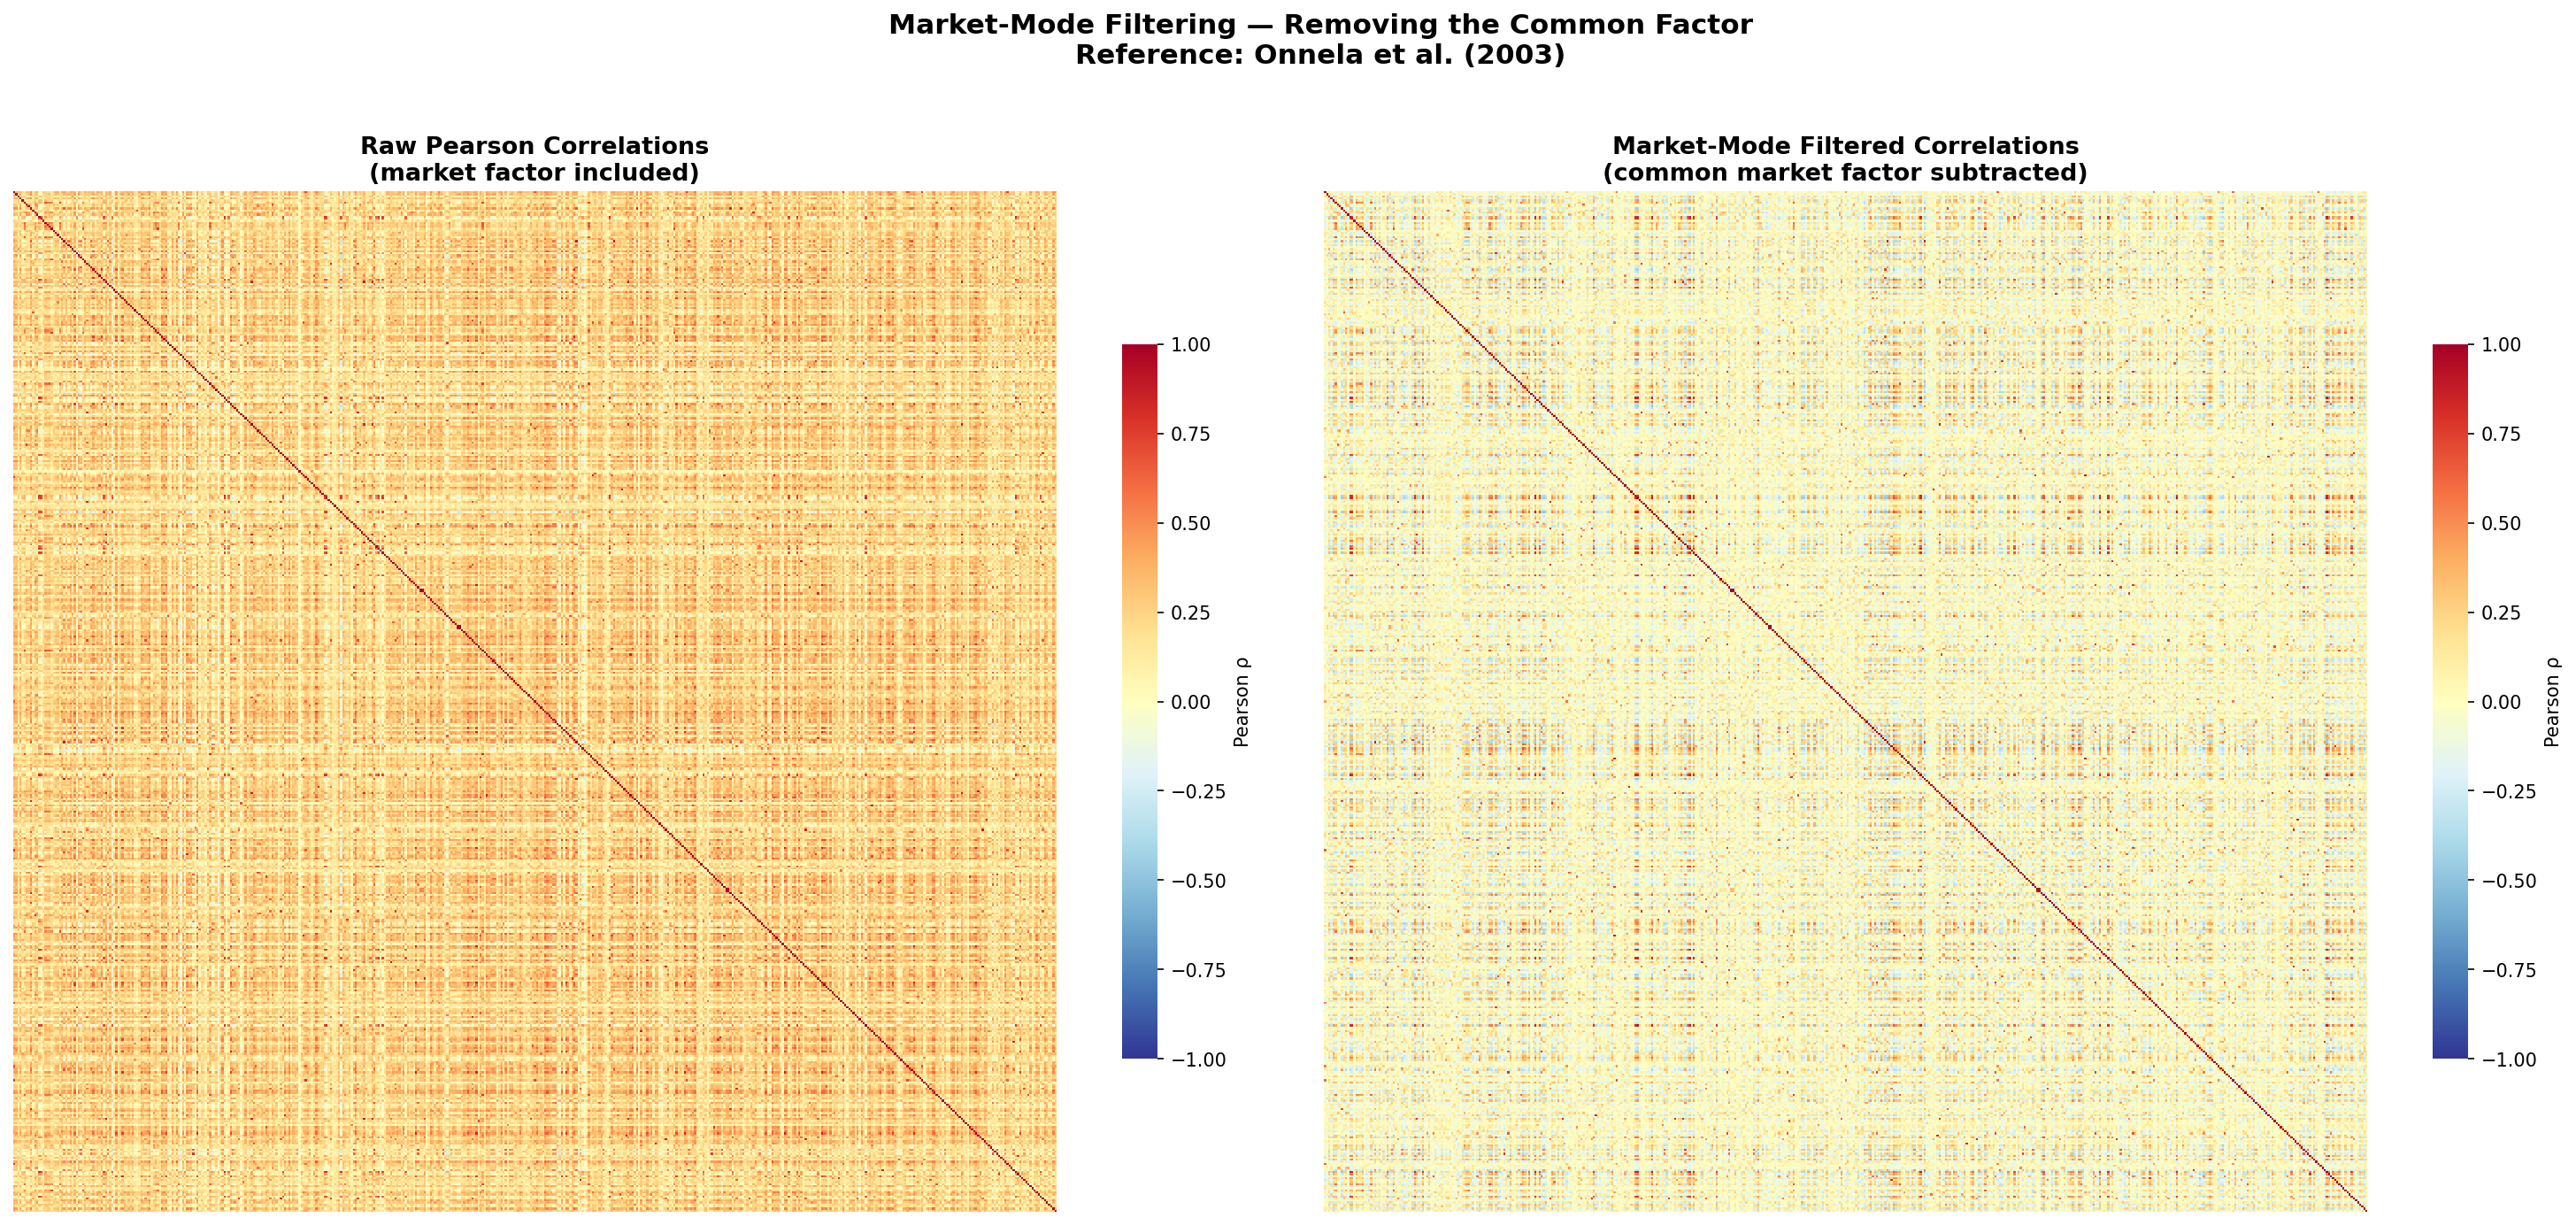
\includegraphics[width=0.88\textwidth]{../../figures/correlation_heatmap_comparison.png}
    \caption{Correlation heatmaps before (left) and after (right) market-mode filtering. The raw matrix shows pervasive positive correlation; the filtered matrix reveals localised modular structure.}
    \label{fig:heatmap}
\end{figure}

\begin{figure}[H]
    \centering
    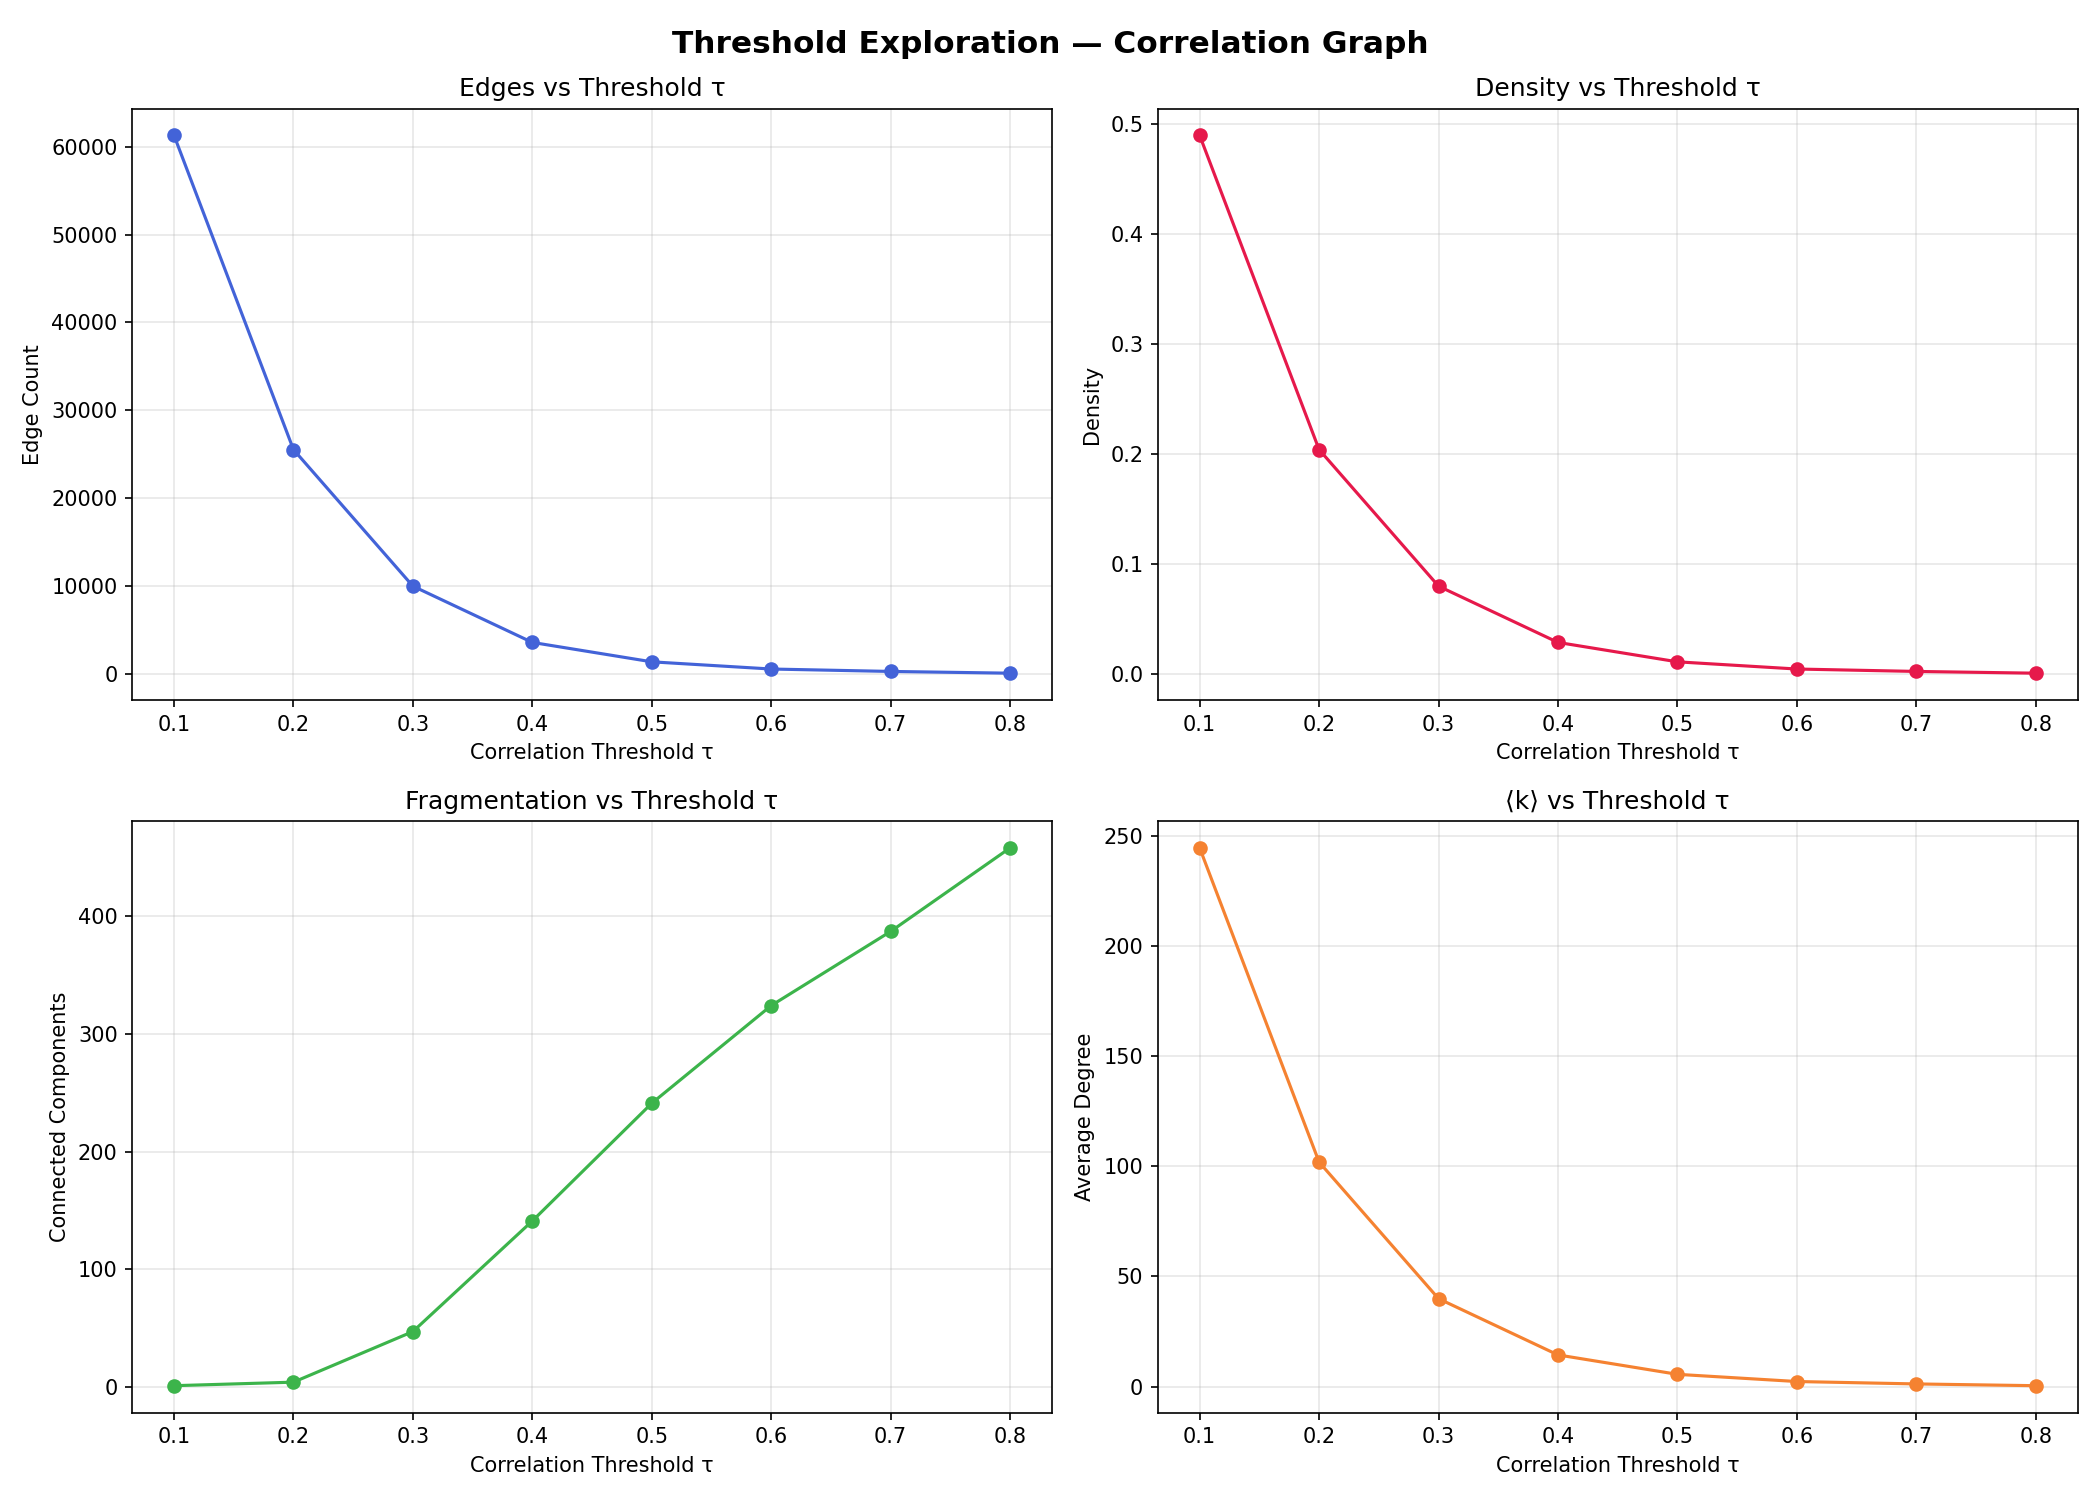
\includegraphics[width=0.65\textwidth]{../../figures/threshold_exploration.png}
    \caption{Edge count, density, number of connected components, and average degree as functions of the correlation threshold $\tau$.}
    \label{fig:threshold}
\end{figure}

\subsection{Minimum Spanning Tree}
A Minimum Spanning Tree (MST) is also constructed using the Mantegna distance~\citep{mantegna1999hierarchical}:
\begin{equation}
    d_{ij} = \sqrt{2(1 - \rho_{ij})},
\end{equation}
which maps correlations into a metric space. The MST extracts the $N-1$ most important links, providing a hierarchical backbone of the market.

% ===================================================================
\section{Scale-Free Analysis}
% ===================================================================

\subsection{Degree Distribution}
The filtered network contains 47 connected components. The Giant Connected Component (GCC) encompasses $448/501 = 89.4\%$ of all nodes.

The degree distribution $P(k)$ is heavy-tailed. Using maximum-likelihood estimation with the \texttt{powerlaw} package~\citep{clauset2009power}, a power-law model is fitted:
\begin{equation}
    P(k) \sim k^{-\gamma}, \quad k \geq k_{\min}.
\end{equation}
The estimated exponent is $\gamma \approx 2.14 \pm 0.58$ (bootstrap $B=200$), placing the network in the scale-free regime $2 < \gamma < 3$~\citep{barabasi2016network}. Likelihood-ratio tests confirm that the power-law fits the tail better than an exponential ($R > 0$, $p < 0.05$), though it is not clearly distinguishable from a log-normal.

\begin{figure}[H]
    \centering
    
\includegraphics[width=0.65\textwidth]{../../figures/powerlaw_fit.png}
    \caption{Empirical degree PDF and CCDF with power-law fit ($\gamma \approx 2.14$). The heavy tail confirms the presence of high-degree hub nodes.}
    \label{fig:powerlaw}
\end{figure}

\subsection{Centrality}
Five centrality measures are computed on the GCC:

\begin{itemize}
    \item \textbf{Degree centrality}: $C_D(i) = k_i / (N-1)$.
    \item \textbf{Weighted degree}: sum of absolute edge weights incident to $i$.
    \item \textbf{Betweenness centrality}: fraction of shortest paths passing through $i$~\citep{freeman1977set}.
    \item \textbf{Eigenvector centrality}: leading eigenvector of the adjacency matrix~\citep{bonacich1987power}.
    \item \textbf{Closeness centrality}: inverse of mean shortest-path distance from $i$ to all other nodes.
\end{itemize}

Utilities-sector companies (Consolidated Edison, Duke Energy, Southern Company) dominate all centrality rankings, reflecting their dense correlation structure driven by shared sensitivity to interest rates and regulatory environments.

% ===================================================================
\section{Small-World}
% ===================================================================

A network is \emph{small-world} if it combines high clustering with short average path lengths relative to a random benchmark~\citep{watts1998collective}. The small-world coefficient~\citep{humphries2008network} is defined as
\begin{equation}
    \sigma = \frac{C / C_{\text{rand}}}{L / L_{\text{rand}}},
\end{equation}
where $C$ and $L$ are the clustering coefficient and average shortest-path length of the empirical GCC, and $C_{\text{rand}}$, $L_{\text{rand}}$ are averages over random null-model graphs.

\subsection{Erd\H{o}s--R\'enyi Baseline}
Using Erd\H{o}s--R\'enyi $G(n,p)$ graphs with matching $n$ and edge probability $p$:
\begin{align}
    C &= 0.643, \quad L = 2.703, \\
    C_{ER} &= 0.100, \quad L_{ER} = 1.911, \\
    \sigma_{ER} &= \frac{0.643 / 0.100}{2.703 / 1.911} = 4.56.
\end{align}

\subsection{Configuration Model Baseline}
The ER model ignores degree heterogeneity. A stricter test uses the configuration model~\citep{molloy1995critical}, which generates random graphs preserving each node's exact degree $k_i$:
\begin{align}
    C_{\text{config}} &= 0.306, \quad L_{\text{config}} = 2.251, \\
    \sigma_{\text{config}} &= \frac{0.643 / 0.306}{2.703 / 2.251} = 1.75.
\end{align}
Since $\sigma_{\text{config}} > 1$, the financial network exhibits small-world clustering \emph{beyond} what degree heterogeneity alone would produce.

\begin{figure}[H]
    \centering
    
\includegraphics[width=0.65\textwidth]{../../figures/er_comparison.png}
    \caption{Degree distribution of the financial network versus an $ER(n,p)$ null model. The ER graph's Poisson shape confirms the financial graph's heavy-tailed departure from randomness.}
    \label{fig:er}
\end{figure}

\subsection{Bootstrap Significance}
Non-parametric bootstrap resampling ($B=200$) of the log-return matrix is performed: rows (trading days) are resampled with replacement, and the full pipeline (filter $\to$ correlate $\to$ threshold $\to$ compute $\sigma$) is repeated. The resulting distribution of $\sigma$ lies entirely above 1.0, yielding $p < 0.001$ for the null hypothesis $H_0\!: \sigma \leq 1$ (Figure~\ref{fig:bootstrap}).

\begin{figure}[H]
    \centering
    
\includegraphics[width=0.78\textwidth]{../../figures/bootstrap_distributions.png}
    \caption{Bootstrap distributions ($B=200$) for $\sigma$, modularity $Q$, NMI, power-law $\gamma$, clustering $C$, and average path length $L$. Red lines indicate point estimates; dashed lines show 95\% confidence intervals.}
    \label{fig:bootstrap}
\end{figure}

% ===================================================================
\section{Contagion}
% ===================================================================

\subsection{Deterministic Propagation}
A multi-hop contagion model simulates financial distress spreading across the network. Given an initial shock of magnitude $I_0$ at a source node $s$, the impact reaching neighbour $j$ at hop $h$ is
\begin{equation}
    \Delta I_j^{(h)} = \alpha^{h} \cdot I_{\text{parent}} \cdot \tilde{w}(u,j),
\end{equation}
where $\alpha = 0.5$ is a decay factor and $\tilde{w}(u,j) = w(u,j) / \sum_k w(u,k)$ is the row-normalised edge weight. Impacts accumulate additively across hops.

Source nodes are selected dynamically as the top nodes by degree, betweenness, and eigenvector centrality. From the highest-degree node (ED, Consolidated Edison), the cascade reaches 444 of 500 other nodes within 3 hops.

\subsection{SIR Epidemic Model}
Following Barab\'asi (Ch.~10), a stochastic SIR (Susceptible--Infected--Recovered) model is simulated on the network:
\begin{itemize}
    \item Each infected node infects each susceptible neighbour with probability $\beta = 0.3$ per time step.
    \item Each infected node recovers with probability $\mu = 0.1$ per time step.
    \item The basic reproduction number is $R_0 = \beta \langle k \rangle / \mu$.
\end{itemize}
Averaged over 50 Monte Carlo runs, the final epidemic size is $R(\infty) = 87.5\%$, confirming that the hub-dominated topology facilitates rapid viral-like spreading.

% ===================================================================
\section{Event Validation}
% ===================================================================

Rather than simulating abstract shocks, the propagation model is validated against three historical market events:

\begin{enumerate}
    \item \textbf{AI / Semiconductor Rally} (July 2024): technology-sector surge driven by earnings beats from major chipmakers.
    \item \textbf{Yen Carry-Trade Unwind} (August 2024): sharp JPY appreciation triggered forced deleveraging across global equity portfolios.
    \item \textbf{U.S.\ Tariff Shock} (April 2025): broad-based sell-off following announcement of new import duties.
\end{enumerate}

For each event, actual event-day returns are extracted from the log-return matrix. The 10 most-affected stocks serve as contagion seeds, with their real returns used as initial shock magnitudes. The model's predicted post-event impacts are compared against realised cumulative returns over a 5-day observation window using Pearson $r$ and $R^2$.

\begin{figure}[H]
    \centering
    \begin{subfigure}{0.48\textwidth}
        
\includegraphics[width=\textwidth]{../../figures/AI_Semiconductor_Rally_validation.png}
        \caption{AI Rally}
    \end{subfigure}
    \hfill
    \begin{subfigure}{0.48\textwidth}
        
\includegraphics[width=\textwidth]{../../figures/Yen_Carry_Trade_Unwind_validation.png}
        \caption{Yen Unwind}
    \end{subfigure}
    \caption{Scatter plots of model-predicted impact versus actual 5-day post-event returns. Each point is one stock, coloured by GICS sector. The regression line and $R^2$ are shown.}
    \label{fig:validation}
\end{figure}

% ===================================================================
\section{Community Structure}
% ===================================================================

\subsection{Louvain Partition}
Community detection is performed using the Louvain algorithm~\citep{blondel2008fast}, which greedily maximises the modularity
\begin{equation}
    Q = \frac{1}{2m} \sum_{ij} \left[ A_{ij} - \frac{k_i k_j}{2m} \right] \delta(c_i, c_j),
\end{equation}
where $A_{ij}$ is the adjacency matrix, $k_i$ is the degree of node $i$, $m$ is the total number of edges, and $\delta(c_i, c_j) = 1$ if nodes $i$ and $j$ belong to the same community.

The algorithm partitions the network into 57 communities with $Q = 0.27$.

\subsection{Comparison with GICS Sectors}
The agreement between Louvain communities and the 11 official GICS sectors is quantified by the Normalised Mutual Information~\citep{danon2005comparing}:
\begin{equation}
    NMI(X, Y) = \frac{2 \, I(X;Y)}{H(X) + H(Y)},
\end{equation}
where $I(X;Y)$ is the mutual information and $H(\cdot)$ is the entropy. The measured $NMI = 0.45$ indicates partial alignment: network communities partially recover sector boundaries but also reveal cross-sector groupings driven by supply-chain linkages and shared factor exposures.

\begin{figure}[H]
    \centering
    \begin{subfigure}{0.48\textwidth}
        
\includegraphics[width=\textwidth]{../../figures/community_detection.png}
        \caption{Network coloured by Louvain community.}
    \end{subfigure}
    \hfill
    \begin{subfigure}{0.48\textwidth}
        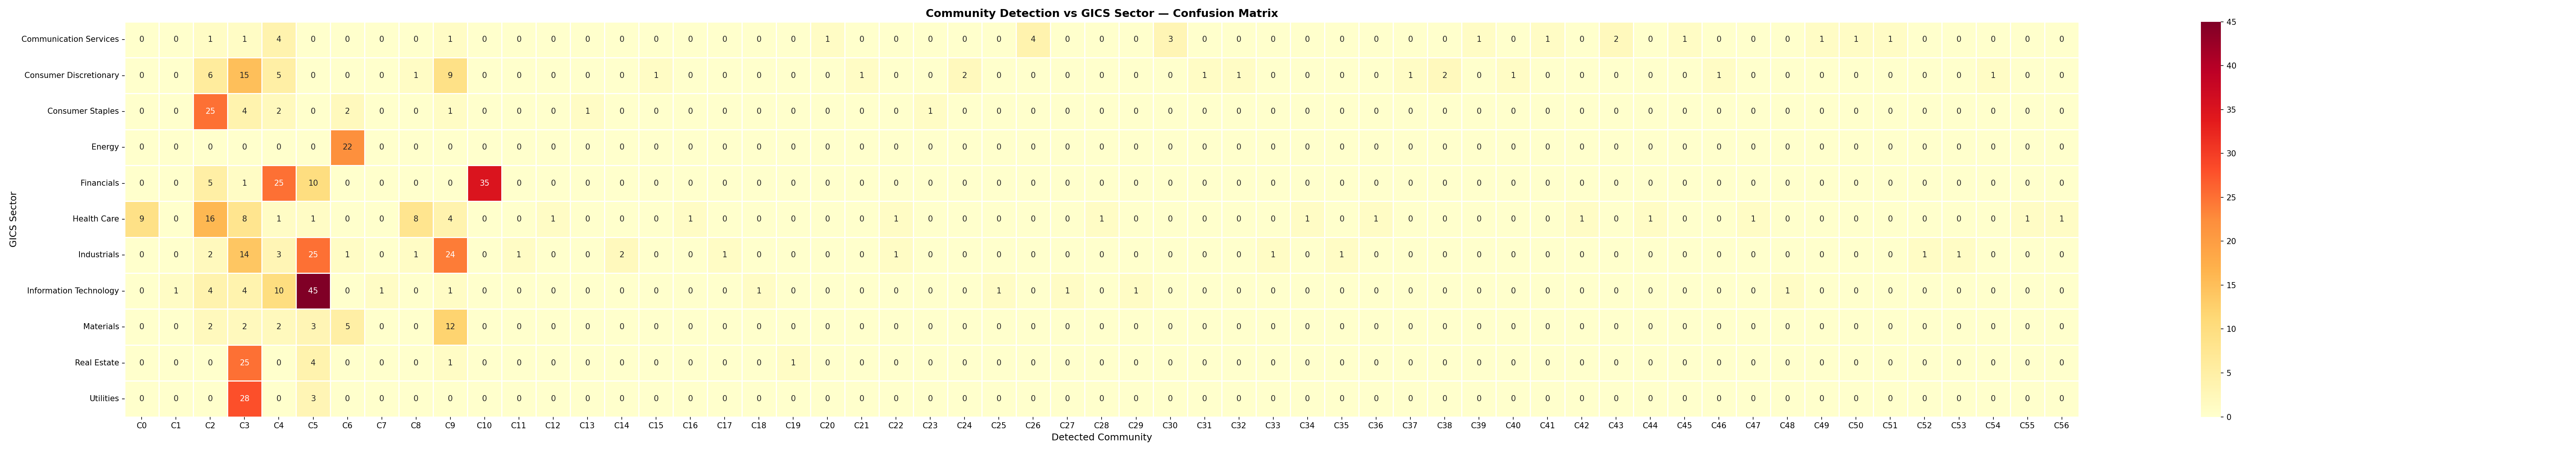
\includegraphics[width=\textwidth]{../../figures/community_vs_sector.png}
        \caption{Community vs.\ GICS sector confusion matrix.}
    \end{subfigure}
    \caption{Louvain communities (57 groups, $Q = 0.27$) versus official GICS sector classification ($NMI = 0.45$).}
    \label{fig:communities}
\end{figure}

\subsection{Influence Leakage}
For the most central node in each sector, influence propagation is run and the fraction of total impact absorbed by same-sector versus cross-sector nodes is computed. On average, 86\% of influence leaks across sector boundaries, confirming strong cross-sector contagion pathways.

% ===================================================================
\section{Robustness}
% ===================================================================

Network robustness is assessed by progressively removing nodes and tracking the relative size of the GCC~\citep{albert2000error, barabasi2016network}:

\begin{enumerate}
    \item \textbf{Random failure}: nodes removed uniformly at random (averaged over 3 trials).
    \item \textbf{Targeted attack (degree)}: nodes removed in decreasing order of degree centrality.
    \item \textbf{Targeted attack (betweenness)}: nodes removed in decreasing order of betweenness, recomputed after each removal.
    \item \textbf{ER baseline}: same procedure on an $ER(n,p)$ graph.
    \item \textbf{Configuration model baseline}: same procedure on a degree-preserving random graph.
\end{enumerate}

\begin{figure}[H]
    \centering
    
\includegraphics[width=0.65\textwidth]{../../figures/robustness_analysis.png}
    \caption{GCC fraction versus fraction of nodes removed under five attack strategies. The financial network is resilient to random failure but collapses rapidly under targeted betweenness attack.}
    \label{fig:robustness}
\end{figure}

Under random failure, the GCC degrades gracefully---a hallmark of scale-free resilience~\citep{albert2000error}. Under targeted betweenness attack, the GCC collapses after removing fewer than 20\% of nodes, exposing the network's dependence on a small number of bridging firms.

% ===================================================================
\section{Temporal Dynamics}
% ===================================================================

Financial networks are non-stationary: correlations shift with market regimes, monetary policy, and geopolitical events. To capture this, 18 overlapping rolling windows of 6 months each are constructed. For each window, the full pipeline (filter $\to$ correlate $\to$ threshold $\to$ build graph) is executed, and the following metrics are tracked:

\begin{itemize}
    \item Mean absolute correlation $\langle |\rho| \rangle$
    \item Edge count and density
    \item Modularity $Q$ and number of communities
    \item Clustering coefficient $C$, average path length $L$, and $\sigma$
\end{itemize}

\begin{figure}[H]
    \centering
    
\includegraphics[width=0.78\textwidth]{../../figures/rolling_window_metrics.png}
    \caption{Evolution of structural metrics across 18 rolling windows. Clustering and modularity increase during stress periods, consistent with a ``flight to correlation'' effect.}
    \label{fig:rolling}
\end{figure}

The results show that during stress periods (e.g., the August 2024 carry-trade crisis), clustering and modularity spike as correlations tighten, while the network becomes denser and more connected. This ``flight to correlation'' aligns with established empirical findings in financial network literature.

% ===================================================================
\section{Conclusions}
% ===================================================================

\begin{table}[H]
\centering
\caption{Summary of key network metrics.}
\begin{tabular}{ll}
\toprule
\textbf{Metric} & \textbf{Value} \\
\midrule
Nodes & 501 \\
Edges (filtered, $\tau = 0.3$) & 10,002 \\
Density & 7.9\% \\
Connected components & 47 \\
GCC fraction & 89.4\% \\
Power-law $\gamma$ & $2.14 \pm 0.58$ \\
Clustering $C$ & 0.643 \\
Avg.\ path length $L$ & 2.703 \\
$\sigma_{ER}$ & 4.56 \\
$\sigma_{\text{config}}$ & 1.75 \\
Louvain communities & 57 \\
Modularity $Q$ & 0.27 \\
NMI (vs.\ GICS) & 0.45 \\
Cross-sector leakage & 86\% \\
Rolling windows & 18 \\
Bootstrap resamples & 200 \\
\bottomrule
\end{tabular}
\end{table}

The S\&P 500 correlation network, after market-mode filtering, is scale-free, small-world, and highly modular. Its topology is resilient to random failures but vulnerable to targeted removal of high-betweenness bridging nodes. Community structure partially aligns with official sector classifications but reveals significant cross-sector dependencies. Rolling-window analysis confirms that these structural properties are dynamic, tightening during periods of market stress. The propagation model, validated against three historical events, demonstrates that network topology captures meaningful information about how shocks propagate through the financial system.

% ===================================================================
% References
% ===================================================================
\begin{thebibliography}{99}

\bibitem[Albert et al.(2000)]{albert2000error}
Albert, R., Jeong, H. and Barab\'asi, A.-L. (2000).
\newblock Error and attack tolerance of complex networks.
\newblock \emph{Nature}, 406(6794), 378--382.

\bibitem[Barab\'asi(2016)]{barabasi2016network}
Barab\'asi, A.-L. (2016).
\newblock \emph{Network Science}.
\newblock Cambridge University Press.

\bibitem[Blondel et al.(2008)]{blondel2008fast}
Blondel, V.~D., Guillaume, J.-L., Lambiotte, R. and Lefebvre, E. (2008).
\newblock Fast unfolding of communities in large networks.
\newblock \emph{Journal of Statistical Mechanics}, 2008(10), P10008.

\bibitem[Bonacich(1987)]{bonacich1987power}
Bonacich, P. (1987).
\newblock Power and centrality: A family of measures.
\newblock \emph{American Journal of Sociology}, 92(5), 1170--1182.

\bibitem[Clauset et al.(2009)]{clauset2009power}
Clauset, A., Shalizi, C.~R. and Newman, M.~E.~J. (2009).
\newblock Power-law distributions in empirical data.
\newblock \emph{SIAM Review}, 51(4), 661--703.

\bibitem[Danon et al.(2005)]{danon2005comparing}
Danon, L., D\'iaz-Guilera, A., Duch, J. and Arenas, A. (2005).
\newblock Comparing community structure identification.
\newblock \emph{Journal of Statistical Mechanics}, 2005(09), P09008.

\bibitem[Freeman(1977)]{freeman1977set}
Freeman, L.~C. (1977).
\newblock A set of measures of centrality based on betweenness.
\newblock \emph{Sociometry}, 40(1), 35--41.

\bibitem[Humphries and Gurney(2008)]{humphries2008network}
Humphries, M.~D. and Gurney, K. (2008).
\newblock Network `small-world-ness': a quantitative method for determining canonical network equivalence.
\newblock \emph{PLOS ONE}, 3(4), e0002051.

\bibitem[Mantegna(1999)]{mantegna1999hierarchical}
Mantegna, R.~N. (1999).
\newblock Hierarchical structure in financial markets.
\newblock \emph{European Physical Journal B}, 11, 193--197.

\bibitem[Mantegna and Stanley(1999)]{mantegna1999introduction}
Mantegna, R.~N. and Stanley, H.~E. (1999).
\newblock \emph{An Introduction to Econophysics}.
\newblock Cambridge University Press.

\bibitem[Molloy and Reed(1995)]{molloy1995critical}
Molloy, M. and Reed, B. (1995).
\newblock A critical point for random graphs with a given degree sequence.
\newblock \emph{Random Structures \& Algorithms}, 6(2--3), 161--180.

\bibitem[Onnela et al.(2003)]{onnela2003dynamics}
Onnela, J.-P., Chakraborti, A., Kaski, K., Kert\'esz, J. and Kanto, A. (2003).
\newblock Dynamics of market correlations: taxonomy and portfolio analysis.
\newblock \emph{Physical Review E}, 68(5), 056110.

\bibitem[Watts and Strogatz(1998)]{watts1998collective}
Watts, D.~J. and Strogatz, S.~H. (1998).
\newblock Collective dynamics of `small-world' networks.
\newblock \emph{Nature}, 393(6684), 440--442.

\end{thebibliography}

\end{document}
